% Drawing 154/02-21 -- folder 154, batch 02, archive page 32 (PDF page 33).
% Transcription: figures dans la marge de la seconde colonne : un disque au bord vert foncé, rayonné de quatre traits vert clair issus d'un point intérieur, quatre petits arcs foncés sur le bord ; au-dessus, un petit polygone colorié en vert, marqué $t$ à droite et $s$ au-dessous, une flèche courbe vers le disque
% Kind: disk with four rays; small polygon above. Method 2 (schematic redraw from the facsimile). Status: partial.
% Notes: Disk: dark green rim, four light green rays from one inner point to the rim, four short dark arcs on the rim (the corners taken off), one in each sector. Above it a small quadrilateral coloured light green and overdrawn with black strokes, t on its right, s below it, a curved arrow from the polygon towards the top of the disk. The black strokes inside the small polygon are not resolved and are left out; its outline is approximate. Redrawn 2026-11-12 (issue 128): to check again. 2026-11-14, Claude Opus 5.5, overlay check (issue 147): rasterised from its own coordinates over the 400 dpi colour scan on a unit grid and measured against the colour masks of the ink; not compiled (no TeX in the session); the redraw is unchanged. The four light green rays and the dark green rim lie on their ink to within about 1 to 2 units (three of the six green strokes are more than 1 unit off over part of their length). Stays partial: the small polygon is a light green patch overdrawn with black zigzag strokes on the page; its outline is drawn as a plain pentagon and the black strokes are left out, and whether they strike the polygon out is not settled.
% Coordinates: 1 unit = 1 mm = 1/100 of the crop width (bbox in page fractions: [0.525, 0.205, 0.63, 0.325]).
% Redrawn by Claude (claude-fable-5-2), issue #128, 2026-11-12; not checked by a human; not compiled (no TeX in the session).
% Checked by Claude (claude-opus-5-5) 2026-11-14 (issue #147): overlaid on the 400 dpi colour facsimile; not compiled (no TeX in the session). Not checked by a human. Status: partial.
% Rights: reproduces part of the work -- behind RENDER_TRANSCRIPTS, never published by itself.
\documentclass[tikz,border=3pt]{standalone}
\usepackage{amsmath,amssymb}
\usetikzlibrary{patterns,arrows.meta}
\tikzset{Lg/.style={green!60!black!70}, Dg/.style={green!45!black}, pencil/.style={black!45}, struck/.style={black!35}, mpt/.style={circle,draw,inner sep=1.3pt}, pt/.style={circle,fill,inner sep=0.9pt}, opt/.style={circle,draw,fill=white,inner sep=1.1pt}}
\begin{document}
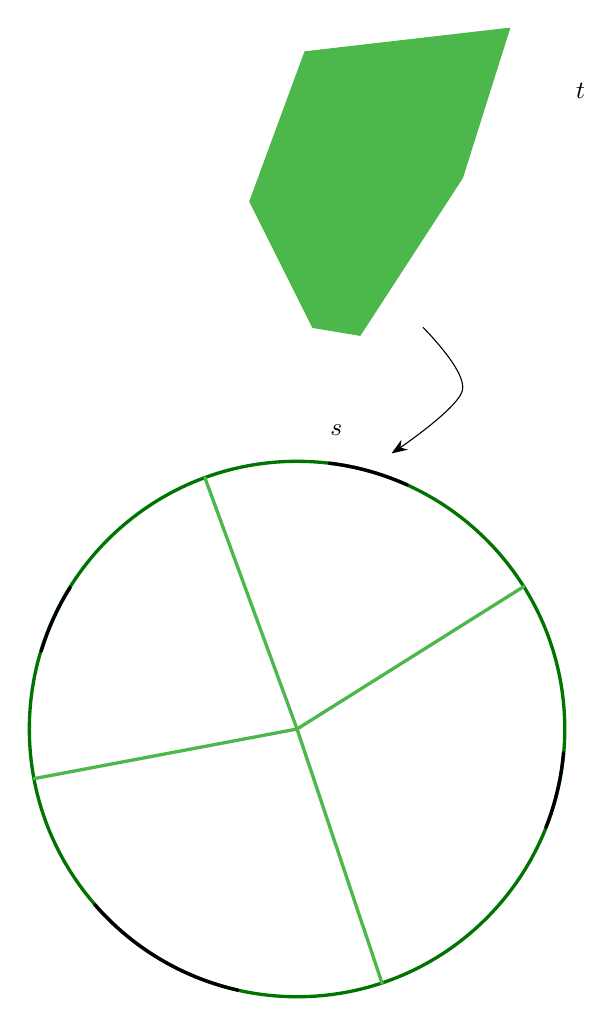
\begin{tikzpicture}[x=1mm,y=1mm,line cap=round,line join=round,font=\scriptsize]
\draw[Dg,very thick] (52,-117) circle[radius=34];
\draw[Lg,very thick] (52,-117) -- (40.3,-85.1);
\draw[Lg,very thick] (52,-117) -- (80.8,-98.9);
\draw[Lg,very thick] (52,-117) -- (18.6,-123.3);
\draw[Lg,very thick] (52,-117) -- (62.8,-149.3);
\draw[very thick] (66,-86) arc[start angle=65.7, end angle=83.1, x radius=34, y radius=34];
\draw[very thick] (23.2,-99) arc[start angle=148, end angle=163.1, x radius=34, y radius=34];
\draw[very thick] (83.6,-129.5) arc[start angle=338.5, end angle=355, x radius=34, y radius=34];
\draw[very thick] (26.3,-139.3) arc[start angle=221, end angle=257.3, x radius=34, y radius=34];
\fill[pattern=north east lines,Lg] (46,-50) -- (53,-31) -- (79,-28) -- (73,-47) -- (60,-67) -- (54,-66) -- cycle;
\draw[Lg] (46,-50) -- (53,-31) -- (79,-28) -- (73,-47) -- (60,-67) -- (54,-66) -- cycle;
\draw[-{Stealth[length=2mm]}] plot[smooth, tension=0.55] coordinates {(68,-66) (73,-74) (64,-82)};
\node[inner sep=1pt] at (88,-36) {\small $t$};
\node[inner sep=1pt] at (57,-79) {\small $s$};
\end{tikzpicture}
\end{document}
